\documentclass[final]{beamer}
\usepackage[size=a0,scale=1.2]{beamerposter}
\usepackage[spanish]{babel}
\usepackage{graphicx}
\usepackage{amsmath,amssymb}
\usepackage{multicol}
\usepackage{color}

\usetheme{Madrid}

\title{Belleza Matemática: Explorando la Estética en los Conceptos Numéricos}
\author{Brenda Vargas Parra}
\institute{Universidad XYZ}

\begin{document}
\begin{frame}[t]

\begin{columns}[t]

%-------------------- COLUMNA 1 ---------------------
\begin{column}{0.48\textwidth}

\begin{block}{Introducción}
La belleza ha sido históricamente asociada con el arte, la música y la literatura, pero también tiene un lugar profundo en las matemáticas. Ciertos teoremas, fórmulas y patrones han sido reconocidos por su elegancia y simplicidad. Un ejemplo representativo es la identidad de Euler:
\[
e^{i\pi} + 1 = 0
\]
Esta ecuación une cinco constantes fundamentales y genera asombro por su armonía.
\end{block}

\begin{block}{¿Qué es la belleza matemática?}
Existen distintas teorías:
\begin{itemize}
    \item \textbf{Objetiva:} belleza inherente a proporciones y simetría.
    \item \textbf{Subjetiva:} depende de la percepción individual.
    \item \textbf{Funcionalista:} belleza ligada a la eficacia estructural.
\end{itemize}
Hardy y Weyl defienden una belleza basada en estructura; Sinclair y Rota resaltan intuición, inevitabilidad y emoción.
\end{block}

\begin{block}{Cualidades estéticas comunes}
\begin{itemize}
    \item Simplicidad: expresividad con pocos elementos.
    \item Simetría: equilibrio interno.
    \item Profundidad: conexiones ocultas.
    \item Sorpresa: descubrimientos inesperados.
    \item Aplicabilidad: descripción elegante del mundo físico.
\end{itemize}
\end{block}

\end{column}

%-------------------- COLUMNA 2 ---------------------
\begin{column}{0.48\textwidth}

\begin{block}{Contexto cultural y percepción}
La percepción de belleza matemática varía entre culturas y épocas:
\begin{itemize}
    \item \textbf{Grecia antigua:} armonía geométrica.
    \item \textbf{Mundo árabe y chino:} patrones algebraicos.
    \item \textbf{Matemática contemporánea:} abstracción, unificación teórica.
\end{itemize}
Un estudiante puede maravillarse ante el triángulo de Pascal, mientras que un matemático ve en él conexiones profundas con combinatoria y probabilidad.
\end{block}

\begin{block}{Relación con el arte}
Matemáticas y arte comparten elementos como:
\begin{itemize}
    \item \textbf{Simetría y orden visual}
    \item \textbf{Proporción áurea}
    \item \textbf{Capacidad de provocar emoción}
\end{itemize}
Aunque el arte busca expresar subjetividad y emoción, y las matemáticas estructura y precisión, ambas pueden ser bellas y evocadoras.
\end{block}

\end{column}
\end{columns}

%---------------------- IMÁGENES (FUERA DE LAS COLUMNAS) -----------------------

\vspace{1cm}

\begin{center}
\begin{minipage}[t]{0.32\textwidth}
    \centering
    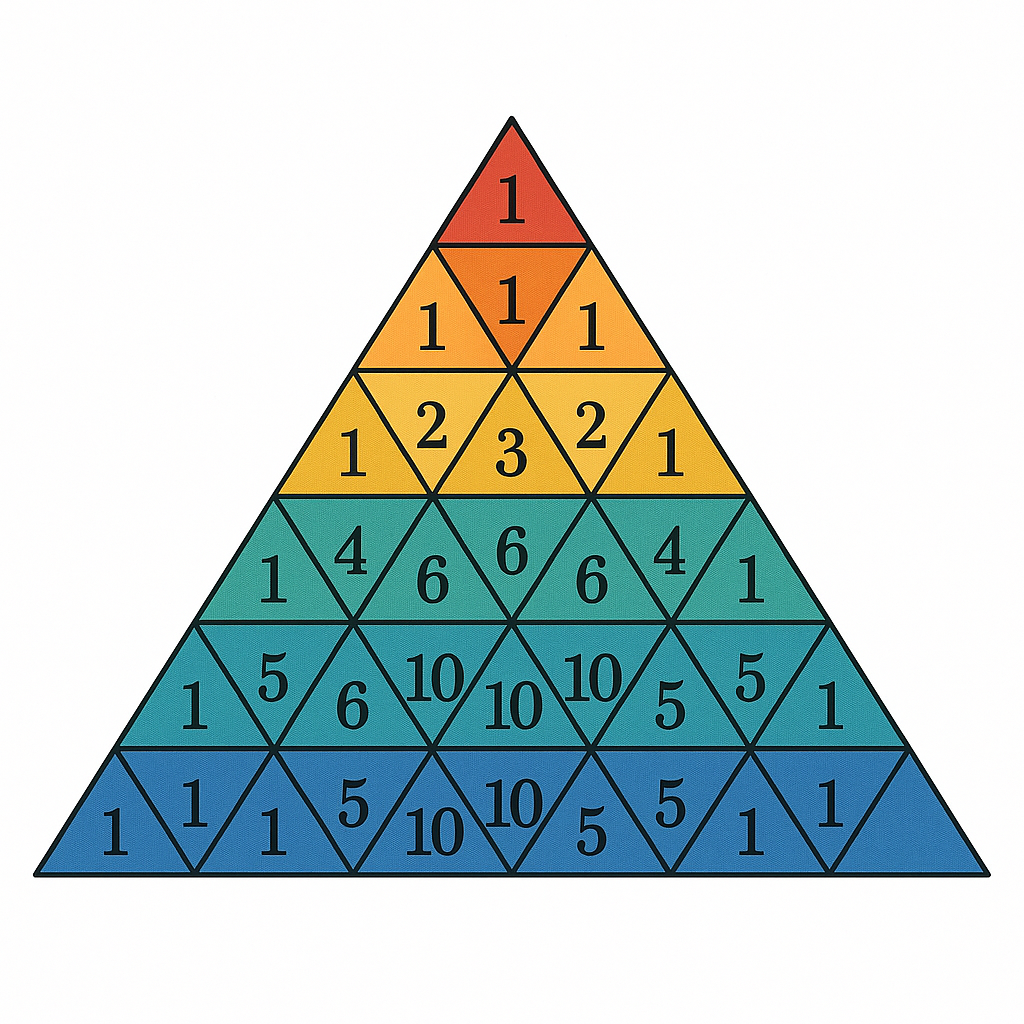
\includegraphics[width=0.95\linewidth]{imagen4.png}\\
    \small Triángulo de Pascal
\end{minipage}
\hfill
\begin{minipage}[t]{0.32\textwidth}
    \centering
    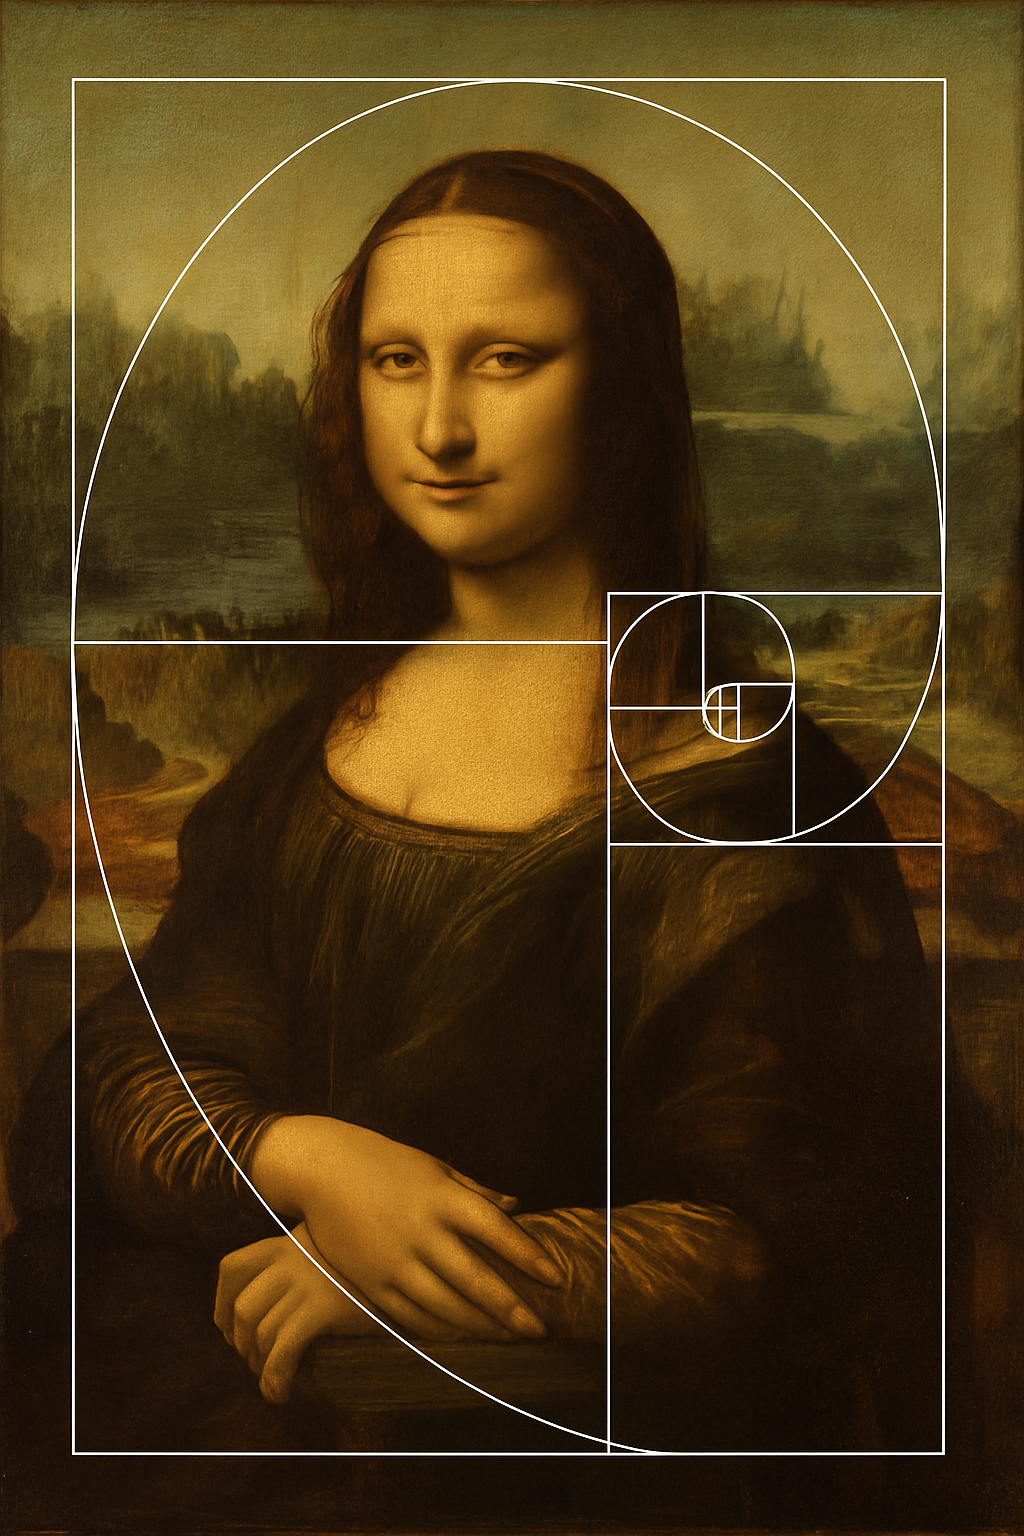
\includegraphics[width=0.8\linewidth]{imagen5.png}\\
    \small Proporción áurea en el arte
\end{minipage}
\hfill
\begin{minipage}[t]{0.32\textwidth}
    \centering
    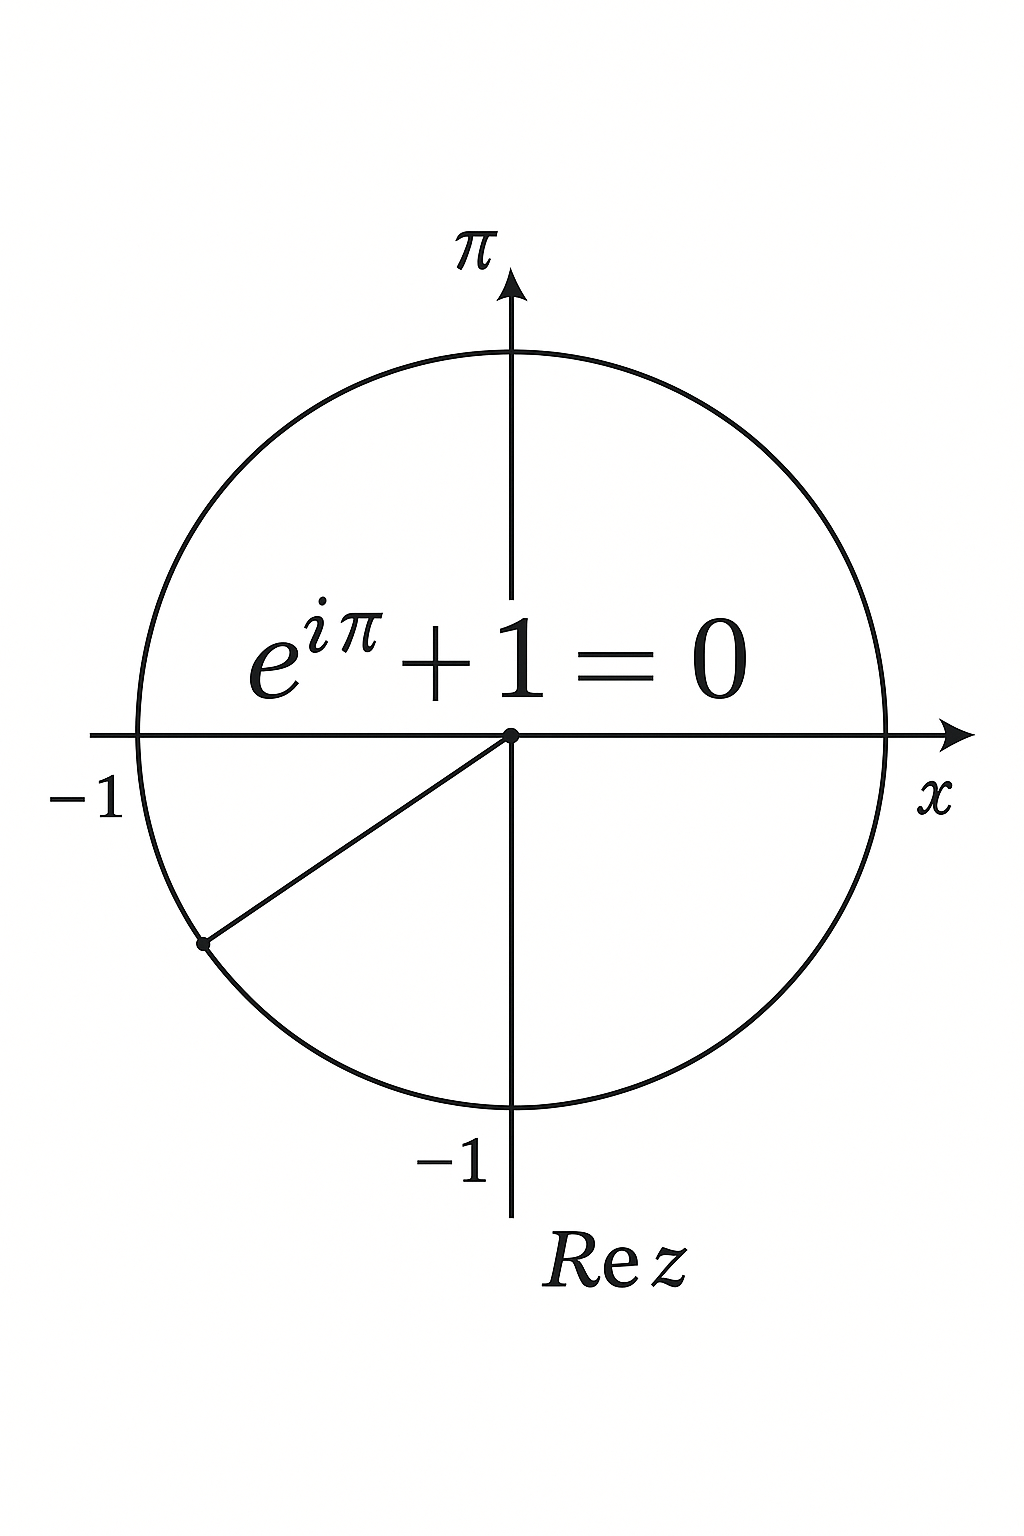
\includegraphics[width=0.8\linewidth]{imagen2.png}\\
    \small Identidad de Euler
\end{minipage}
\end{center}

\vspace{1cm}


\vspace{1.5cm}
\begin{block}{Conclusión}
La belleza matemática trasciende lo lógico y se convierte en una experiencia estética. Surge tanto de su forma estructural como del asombro que despierta en quien la contempla. Matemáticas y arte no son opuestos: comparten el anhelo de revelar armonía y verdad a través de distintos lenguajes. Comprender esta belleza nos permite ver el pensamiento abstracto como una forma de creación tan profunda como una obra de arte.
\end{block}

\end{frame}
\end{document}
